\documentclass[12pt,a4j]{article}
\usepackage{fontspec}
\setmainfont{Arial}
\def\Vec#1{\mbox{\boldmath $#1$}}
\usepackage[dvipdfmx]{graphicx}

\setlength{\textheight}{275mm}
\headheight 5mm
\topmargin -20mm
\textwidth 160mm
\textheight 250mm
\oddsidemargin -0mm
\evensidemargin -5mm

\pagestyle{empty}
\makeatletter
  \def\@maketitle{%
  \newpage\null
  \vskip 2em%
  \begin{center}%
  \let\footnote\thanks
    {\large\bf \@title \par}%
    \vskip 1.5em%
    {\large\bf \@author \par}%
    \vskip 1.5em%
    {\small \@date}%
  \end{center}%
}
\makeatother

%\documentclass[10pt, a4j]{article}
%%\usepackage{citesort}
\usepackage{amssymb}
\usepackage[dvipdfmx]{graphicx}% 図を入れるときに使用
\usepackage{wrapfig}% 図の周りに本文を流し込みたいときに使用
\usepackage{subfigure}
\usepackage{here}
\begin{document}
\title{Cluster ordering of Mg-LPSO}
\author{Shinya Morishita and Shigeto R. Nishitani}
\date{}
\maketitle
Two possible scinarios, solute ordering and stacking fault induced, have been discucced for the formation mechanisms of the long period stacking ordered (LPSO) structure in Mg based alloys.  Very recently, the authors have reported the solute ordering of mini clusters[1].  In this talk, we will show the first principles calculations of the interaction energy between a $L1_2$ cluster and a mini cluster, and discusses the diffusion mechanism of this mini cluster.

\begin{wrapfigure}{r}{8cm}
\vspace{-8\baselineskip}
\begin{center}
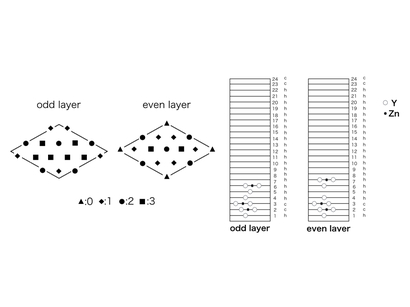
\includegraphics[width=6cm,bb=0 0 442 500]{../figs/./calphad_donkey.001.jpeg}
\caption{Schematic drawings of slab models.}
\end{center}
\vspace{0\baselineskip}
\end{wrapfigure}
The target mini cluster was reported by Kiyohara et al.[2], where the horizontally split $L1_2$ cluster shows relatively stable energy in the hcp lattice.  The distance dependency of interaction energy between $L1_2$ cluster and a mini cluster are calculated by VASP.  The calculated models are shown in Fig.1. The marks in the top view indicate the equivalent site of the location of a mini cluster in a- and c- layers of hcp stacking.  

\begin{wrapfigure}{r}{8cm}
\vspace{-7\baselineskip}
\begin{center}
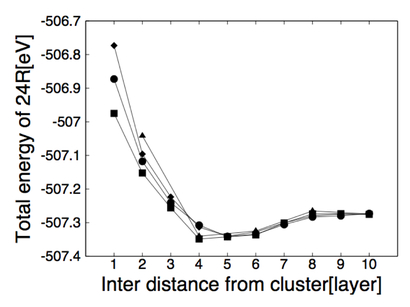
\includegraphics[width=6cm,bb=0 0 442 500]{../figs/./calphad_donkey.002.jpeg}
\caption{Energy dependency on vertical distance between $L1_2$ and mini clusters.}
\end{center}
\vspace{0\baselineskip}
\end{wrapfigure}
Fig.2 shows the total energy changes depending on the vertical distance between $L1_2$ cluster and a mini cluster.  A mini cluster shows a minimum around 4-5 layers, which is abount 0.1eV lower than the far end.  This energy minimum indicates that the solute ordering is a strong candidate to induce the formation of the LPSO structure.

If we accept the energetic stability of solute ordering by a mini cluster, we have to discuss the kinetics of the solute movement. For two possibilities of an isolated solute diffusion or a cluster diffusion, we are calculating the stability of the vacancy and multi-vacancies around the mini cluster.  
\begin{enumerate}
\item S Morishita, M Kiyohara, Y Sakamoto, and S. R. Nishitani, LPSO2016, (Kyoto, 2016).
\item M. Kiyohara, Y. Sakamoto, T. Yoshioka, S. Morishita, and S. R. Nishitani: proceedings of PRICM, (Kyoto 2016).
\end{enumerate}
\end{document}
